\documentclass[border=10pt]{standalone}
\usepackage{tikz,amsmath}
\usetikzlibrary{arrows.meta}

% ========== 配色 ==========
\definecolor{hidFill}{RGB}{199,203,243}
\definecolor{hidLine}{RGB}{52,58,143}
\definecolor{inFill}{RGB}{183,224,177}
\definecolor{inLine}{RGB}{32,102,32}
\definecolor{outFill}{RGB}{243,199,199}
\definecolor{outLine}{RGB}{143,52,52}

\begin{document}
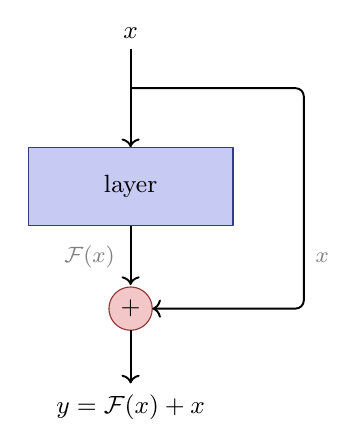
\begin{tikzpicture}[
    font=\small, line join=round,
    every node/.style={inner sep=0pt, outer sep=0pt, align=center},
    fbox/.style={draw=hidLine, fill=hidFill, minimum width=2.6cm, minimum height=1.0cm},
    add/.style ={circle, draw=outLine, fill=outFill, minimum size=.55cm},
    arr/.style ={->, line width=.7pt, rounded corners=3pt}
  ]

  % ================= 输入 x（★ 上移，拉大与框的留白） =================
  \node (xin) at (0,5.8) {$x$};
  \coordinate (s) at (0,5.1);                 % 分叉点：主路向下、旁路绕行
  \draw[arr] (0,5.6) -- (0,4.35);

  % ================= 一个框：layer，输出 F(x) =================
  \node[fbox] (F) at (0,3.85) {layer};
  \draw[arr] (F) -- (0,2.6);
  \node[font=\footnotesize, text=gray, anchor=east] at (-0.2,2.95) {$\mathcal{F}(x)$};

  % ================= 加法器 =================
  \node[add] (ad) at (0,2.3) {+};

  % ================= 旁路：绕过框直接进加法器（★ 标签改为 x） =================
  \draw[arr] (s) -- (2.2,5.1) -- (2.2,2.3) -- (ad.east);
  \node[font=\footnotesize, text=gray, anchor=west] at (2.35,2.95) {$x$};

  % ================= 输出 =================
  \draw[arr] (ad) -- (0,1.35);
  \node at (0,1.05) {$y=\mathcal{F}(x)+x$};

\end{tikzpicture}
\end{document}